%TODO colors
%TODO table at "as follows"
\chapter{CYBERNETIC EYES}\label{CYBERNETIC EYES}
\section*{1. Preamble: About this introductory chapter}
\begin{center}
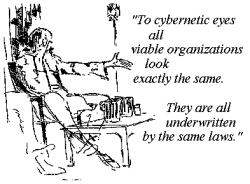
\includegraphics[max width=\textwidth]{sbmugs3_250x184}
\end{center}

This chapter contains a brief introduction to the fundamental ideas on which the Viable Systems Model (or VSM) is based.

The intention is to set the scene, to give you an overview, to sketch out the outline. So don't try and thoroughly understand it all. If you get an idea of how it developed, what it's about and why it's different from most other models, then it's done its job. Consider this chapter as a quick journey through a country you may decide to visit and study at a later date.

In some ways this is the most difficult task. The VSM is very different from anything else I've come across, and the tendency is to miss the whole point and re-interpret it as just another way of looking at the same old ideas of how organisations work.

The difference is that the VSM is a "whole systems" theory. Almost all other theories of organisation think in the billiard-balls mode of A leads to B leads to C, and therefore miss the essence of what's really going on. They forget that A, B and C are inextricably linked with a myriad other factors, and that for any model to work it must take all of this complexity into account.

The VSM is more in tune with other whole systems ideas like acupuncture, the Gaia hypothesis, most of modern physics and many aspects of Eastern religions. The trouble is that most of us see the world in different terms which have their perspectives set by the world-view of Newton and Descartes.

So the job is to provide you with a new way of thinking about organisations which is radically different from traditional, often hierarchical, models ...

The reward of this leap to new ways of thinking is the ability to think about organisations using a rich new language, and actually to be able to do something about problems which may be concerning you.

For this to happen, you have to learn to see the world through cybernetic eyes.

\begin{center}
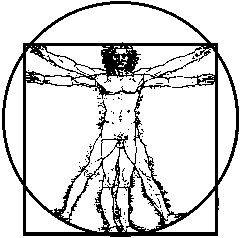
\includegraphics[max width=\textwidth]{v2man100}
\end{center}

\section*{2. The Approach}
During the 1950s Stafford Beer was working as a manager in British Steel and had become dissatisfied with traditional methods of organisation. Rather than attempt to modify what seemed to be a system of fundamentally flawed ideas he took a dramatically fresh approach. He began to study organisations which were obviously several light years ahead in the way they functioned. More specifically, he looked at the way the human brain organises the operation of the muscles and organs.

\textit{"We will seek the source of effective organisation in the cybernetics of natural processes - the brain itself."}

\textbf{We can study the extraordinary beauty of the human form, and base an organisational model on the methods used by the central and autonomic nervous systems to manage the workings of the organs and muscles.}

Beer's studies of the human form, the muscles and organs and all the various nervous systems were the inspiration for the Viable Systems Model.

It may be considered as a generalisation of the way that we all "manage" ourselves in response to a changing environment.

\begin{center}
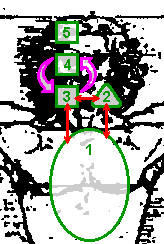
\includegraphics[max width=\textwidth]{1vsm4-1}
\end{center}

\subsection*{Generalisation - The Five Systems}
Beer's studies led him to view the human form as five interacting systems.

\begin{itemize}
  \item \textbf{SYSTEM 1}: All the muscles and organs. The parts that actually DO something. The basic activities of the system. The \textcolor{O}{\textbf{Operation}}.

  \item \textbf{SYSTEM 2}: The sympathetic nervous system which monitors the muscles and organs and ensures that their interaction are kept stable.

  \item \textbf{SYSTEM 3}: The Base Brain which oversees the entire complex of muscles and organs and optimises the internal environment.

  \item \textbf{SYSTEM 4}: The Mid Brain. The connection to the outside world through the senses. Future planning. Projections. Forecasting.

  \item \textbf{SYSTEM 5}: Higher brain functions. Formulation of Policy decisions. Identity.

\end{itemize}

\section*{3. The Three Elements \textcolor{E}{Environment}, \textcolor{O}{Operation}, and \textcolor{M}{Metasystem}}
Beer's first insight was to consider the human organism as three main interacting parts: the muscles \& organs, the nervous systems, and the external environment. Or a little more crudely, body, brain and environment.

These are generalised in the Viable Systems Model as follows:

\begin{tabular}{  p{0.1\textwidth}  p{0.9\textwidth} }
First	&	The \textcolor{O}{\textbf{Operation}}. The muscles and organs. The bits which do all the basic work. The primary activities.\\
\\
Second	&	The \textcolor{M}{\textbf{Metasystem}}. The brain and nervous systems. The parts which ensure that the various Operational units work together in an integrated, harmonious fashion. The job of the \textcolor{M}{\textbf{Metasystem}} is to hold the whole thing together.\\
\\
Third	&	The \textcolor{E}{\textbf{Environment}}. All those parts of the outside world which are of direct relevance to the system in focus.
\end{tabular}

\begin{center}
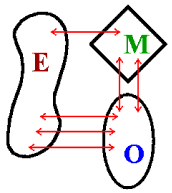
\includegraphics[max width=\textwidth]{vsmbasct}
\end{center}

\section*{Here is a basic VSM diagram}
The \textcolor{E}{\textbf{Environment}} is drawn as an amoeboid shape. The \textcolor{O}{\textbf{Operation}} and \textcolor{M}{\textbf{Metasystem}} are drawn as an ellipse and diamond respectively. (This is taken from Beer's conventions, although I have stretched his Operational circle into an ellipse.) The arrows indicate some of the many and various ways the three elements interact. Each arrow may have several aspects: information (by phone, computer, conversation), movement of trucks, people, money or goods.

{[}Note the approximation involved in drawing these three elements as separate. The \textcolor{E}{\textbf{Environment}} should really go all the way around both the \textcolor{O}{\textbf{Operation}} and its \textcolor{M}{\textbf{Metasystem}}. And the \textcolor{M}{\textbf{Metasystem}} should really be embedded in the \textcolor{O}{\textbf{Operation}}. The teasing apart is necessary to show the way the three elements interact .. {]}

\section*{4. The Three Elements as a Balanced Whole System}
Throughout the discussions which follow it is crucial to bear in mind that the VSM considers an organisation as a whole system which must be in balance with its environment.

This balance is the essence of VSM diagnosis. It's comparable to the approach taken by acupuncture which considers illness as an imbalance in the bodily functions diagnosed by an imbalance in the 12 pulses. Restore the balance - the illness goes away. And just as acupuncture will look at any imbalance between a patient and that patient's environment, so the VSM considers as fundamental the study of an organisation in its environment.

So, although it may be useful to take a limited view of some part of the VSM for a particular purpose, the emphasis will always be on the ecology of an organisation interacting with its environment.

This balanced whole-system approach resolves many of the dilemmas with which traditional models struggle. Should we centralise or decentralise?? Should we devolve power or appoint authoritarian managers??

All these questions will be dealt with as we build up the model. The design of the \textcolor{M}{\textbf{Metasystem}} depends upon the particular conditions within the \textcolor{O}{\textbf{Operation}}. They must be in balance. As the environment changes, the organisation must respond. This will usually require a change in the \textcolor{O}{\textbf{Operation}} to balance the environmental changes and then it's inevitable that the \textcolor{M}{\textbf{Metasystem}} will also have to adapt as it has to be in balance with its \textcolor{O}{\textbf{Operation}}.

All VSM diagnosis, analysis, and discussion is done in this way. The approach relies heavily on drawings and sketches which seem to be the appropriate way to represent a whole system. Quite often a few rough sketches will illuminate a problem which seems intractable when written as an essay.

\section*{5. The Five Systems (Physiological model)}
The Viable Systems Model is composed of the three elements: \textcolor{E}{\textbf{E}}, \textcolor{O}{\textbf{O}} and \textcolor{M}{\textbf{M}}. The \textcolor{O}{\textbf{O}} and \textcolor{M}{\textbf{M}} bits further subdivide into five interacting systems. They were originally derived from Beer's thinking about the "management" of the muscles by the brain and nervous systems.

Consider the following diagram of the central and autonomic nervous systems, shown interacting with both an external environment and (for this example) four muscles and organs.

\begin{center}
	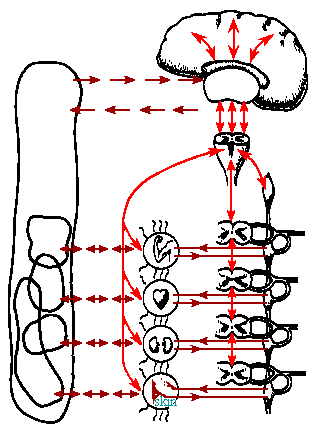
\includegraphics[max width=\textwidth]{pm5sys_}
\end{center}

{\renewcommand{\arraystretch}{1.5} %<- modify value to suit your needs
\begin{tabular}{ | p{0.14\textwidth} | p{0.76\textwidth} | }
	\hline
	\textbf{System 5} & The Cortex. Higher brain functions. \\
	\hline
	\textbf{System 4} & Diencephalon Input from senses, forward planning. \\
	\hline
	\textbf{System 3} & Base brain. Pons and medulla. Internal regulation. \mbox{Optimisation}. \\
	\hline
	\textbf{System 2} & The sympathetic nervous system. Its function is to \mbox{stabilise} the activity of muscles and organs. \\
	\hline
	\textbf{System 1} & Muscles, organs. Primary activities. \\
	\hline
\end{tabular}
}

In their (possibly over-)simplified form the five systems are as follows:

{\renewcommand{\arraystretch}{1.5} %<- modify value to suit your needs
	\begin{tabular}{ | p{0.14\textwidth} | p{0.76\textwidth} | }
		\hline
		\textbf{System 5} & Policy, ultimate authority, identity. \\
		\hline
		\textbf{System 4} & Adaptation, forward planning, strategy. \\
		\hline
		\textbf{System 3} & Internal regulation, optimisation, synergy.  \\
		\hline
		\textbf{System 2} & Conflict resolution, stability. \\
		\hline
		\textbf{System 1} & Primary activities. \\
		\hline
	\end{tabular}
}

These five systems form the basis of the Viable Systems Model. Their functions are general enough to make the model applicable to any and all systems which are viable in that they can maintain a separate existence.

Much of what follows will be discussed in terms of these five systems.

\section*{6. The Five Systems - Creating a Whole from the Parts}
I like to think of the five Systems in terms of what's needed in order to ensure that a number of parts come together to form an integrated whole system. The argument goes like this:

\begin{enumerate}
  \item First of all you need the working bits. This is System 1 (S1) which has previously been called the \textcolor{O}{\textbf{Operation}}. S1 is the bit which actually does something. It's the muscles, the engine room, the machines, the producers.

  \item Secondly you must ensure that there are ways of dealing with conflicting interests which are inevitable in the interactions which occur as the parts of S1 interact. Conflict resolution is the job of System 2. System 2 is also given the job of ensuring stability.

  \item Once the interactions of the System 1 units are rendered stable, it becomes essential to look at ways of \textit{optimising} these interactions. This is the job of System 3. System 3 works with an overview of the entire complex of interacting System 1 units and thinks "If this one does this and that one does that, then the whole thing will work more effectively." The extra efficiency is called synergy. System 3 is there to regulate System 1 - its function is optimisation.

  \item Once you have a stable, optimised set of \textcolor{O}{\textbf{Operation}}al units, then you must ensure that it can survive in a changing environment. This is the job of System 4. System 4 looks at the outside world, considers what it sees, looks for threats and opportunities, and schemes. S4 is there to produce plans to ensure long term viability.

  \item And finally, the whole thing must function within some sort of overall context. Everyone must be pulling in the same direction. This is System 5's job. It provides the ground rules and the means of enforcing them to ensure that the system in complete. System 5 provides the ultimate authority.

\end{enumerate}

\begin{center}
	\textbf{The five systems develop into an extraordinarily powerful model of the way things work.}

	\textbf{The next step is to turn these ideas into a diagram.}
\end{center}

\section*{7. The Five Systems - Graphical Representation}
\textbf{The result is shown below:}

\textbf{In VSM diagnosis you will re-think your organisation in terms of these five systems, and the most powerful approach is to visualise your understanding as a diagram something like the pictures on this page.}

\section*{8. The \textcolor{M}{\textbf{Metasystem}}: a little more detail}

\subsection*{The \textcolor{M}{\textbf{Metasystem}} is there to provide a service.}
In most traditional companies the Metasystemic jobs will be carried out by "higher management" - typically directors. In VSM terms they are only there to service the needs of the Operational parts of the organisation.

Compare this with the traditional view that the Operational parts are only there to carry out the orders of the Directors.

\section*{9. The \textcolor{O}{\textbf{Operation}}: a little more detail}
Whatever your organisation, the Operational part will be composed of sub-units. These are the Operational units. They may be people, or departments, or divisions, or separate companies.

This diagram shows the (large) Operational ellipse, inside which are three (smaller) Operational elements.


\section*{Review - The Form of the Viable Systems Model}
The model is recursive, that is the same principles of organisation \textit{recur} at all organisational levels, regardless of scale. This means that any Viable System is composed of smaller Viable Systems and is embedded in a larger Viable System.
